% ch04_slam.tex
% Chapter 4: Bio-Mimetic SLAM with Sonar Landmarks
% Dr. Yael Mizrahi : LaTeX Technical Author
% XeLaTeX : Hebrew primary, English terms in \en{}

\selectlanguage{hebrew}

\section{SLAM \en{Biomimetic} עם נקודות ציון סונאר}
\label{sec:ch04_slam}

\subsection{ייצוג מפת נקודות ציון}
\label{sec:ch04_landmark_representation}

הדים סונאריים מספקים טווח וכיוון למשטחים מחזירי אור בסביבה. כל הד מזוהה הופך לנקודת ציון תלת-ממדית עם אי-ודאות נלווית, המיוצגת כגאוסיאן עם ממוצע $\boldsymbol{\mu}_j$ וקווריאנס $\boldsymbol{\Sigma}_j$. שיוך נתונים משתמש במרחק \en{Mahalanobis} בין נקודות ציון חזויות לנצפות, עם מבחן סף $\chi^2$ לדחיית חריגים. המערכת שומרת מקסימום של 500 נקודות ציון כדי להגביל את המורכבות החישובית.

ההשראה הביולוגית לייצוג זה מגיעה מה-\en{place cells} הנפחיים בהיפוקמפוס העטלף. שדות הירי האיזוטרופיים ($\sigma \approx 30$ סנטימטרים) מצביעים על כך שיש לייצג נקודות ציון סונאר עם אליפסואידי אי-ודאות כדוריים בערך, בניגוד לאליפסואידים המוארכים האופייניים ל-\en{SLAM} מבוסס ראייה. ייצוג זה מתאים במיוחד למדידות סונאר, שבהן אי-ודאות הטווח קטנה (ס"מ בודדים) אך אי-ודאות הכיוון גדולה (10 עד 20 מעלות).

מטריצת הקווריאנס של נקודת ציון $j$ מיוצגת כ:
\begin{equation}
\boldsymbol{\Sigma}_j = \mathbf{R}_j \cdot \text{diag}(\sigma_r^2, \sigma_\theta^2, \sigma_\phi^2) \cdot \mathbf{R}_j^T
\label{eq:ch04_landmark_cov}
\end{equation}
כאשר $\mathbf{R}_j$ היא מטריצת הסיבוב ממערכת קואורדינטות קוטבית לקרטזית, $\sigma_r$ היא אי-ודאות הטווח (2 ס"מ), $\sigma_\theta$ היא אי-ודאות הזווית האופקית (15 מעלות), ו-$\sigma_\phi$ היא אי-ודאות הזווית האנכית (15 מעלות).

\subsection{שיוך נתונים ומעקב נקודות ציון}
\label{sec:ch04_data_association}

שיוך נתונים בין מדידות סונאר חדשות לנקודות ציון קיימות במפה מתבצע באמצעות מרחק \en{Mahalanobis}:
\begin{equation}
\nu_{ij} = \mathbf{z}_i - h(\hat{\mathbf{x}}, \boldsymbol{\mu}_j), \quad d_{ij}^2 = \nu_{ij}^T \mathbf{S}_{ij}^{-1} \nu_{ij}
\label{eq:ch04_mahalanobis}
\end{equation}
כאשר $\mathbf{z}_i$ היא מדידת הסונאר ה-$i$, $h(\cdot)$ היא פונקציית המדידה, $\hat{\mathbf{x}}$ הוא המצב המשוער של הרחפן, $\boldsymbol{\mu}_j$ הוא מיקום נקודת הציון $j$, ו-$\mathbf{S}_{ij}$ היא קווריאנס החדשנות. מדידה משויכת לנקודת ציון $j$ אם $d_{ij}^2 < \chi^2_{0.95, m}$, כאשר $m$ הוא ממד המדידה.

מעקב נקודות ציון משתמש במסנן \en{nearest neighbor} (\en{NN}) עם חלון אימות. נקודות ציון שלא נצפו במשך $N_{\text{max}} = 10$ מחזורי סונאר מוסרות מהמפה הפעילה אך נשמרות במאגר לזיהוי לולאות סגורות עתידי. גישה זו מונעת התנפחות המפה תוך שמירה על מידע היסטורי לסגירת לולאות.

\subsection{SLAM מבוסס חלקיקים עם מידע דופלר}
\label{sec:ch04_particle_filter_slam}

\en{FastSLAM 2.0} מספק פתרון בר-קנה מידה לבעיית \en{SLAM} על ידי פירוק הפוסטריורי למכפלה של מסנן חלקיקים על מסלולי הרובוט ומסנני \en{EKF} בלתי-תלויים על מיקומי נקודות הציון \cite{Montemerlo2002FastSLAM}. כל חלקיק שומר השערת מסלול ואמידות נקודות ציון משלו. מדידת מהירות הדופלר משפרת את התפלגות ההצעה, ומרכזת חלקיקים באזורים עקביים עם המהירות הנצפית. זה מפחית את מספר החלקיקים הנדרש ($N=50$ לעומת $N=200$ ב-\en{FastSLAM} סטנדרטי) תוך שמירה על דיוק אמידה.

התפלגות ההצעה האופטימלית ב-\en{FastSLAM 2.0} משלבת את המדידה הנוכחית:
\begin{equation}
\pi(\mathbf{x}_k | \mathbf{x}_{k-1}, \mathbf{z}_k, \mathbf{u}_k, \mathbf{m}_{k-1}) = p(\mathbf{x}_k | \mathbf{x}_{k-1}, \mathbf{u}_k, \mathbf{z}_k, \mathbf{m}_{k-1})
\label{eq:ch04_proposal}
\end{equation}
זה מקטין את השונות של משקלי החלקיקים ומונע התנוונות. משקל העדכון של חלקיק $i$ הוא:
\begin{equation}
w_k^{(i)} = w_{k-1}^{(i)} \cdot \frac{p(\mathbf{z}_k | \mathbf{x}_k^{(i)}, \mathbf{m}_{k-1}^{(i)}) \cdot p(\mathbf{x}_k^{(i)} | \mathbf{x}_{k-1}^{(i)}, \mathbf{u}_k)}{\pi(\mathbf{x}_k^{(i)} | \mathbf{x}_{k-1}^{(i)}, \mathbf{z}_k, \mathbf{u}_k, \mathbf{m}_{k-1}^{(i)})}
\label{eq:ch04_weight_update}
\end{equation}

\subsection{עדכון נקודות ציון ב-EKF}
\label{sec:ch04_landmark_ekf}

כל חלקיק ב-\en{FastSLAM 2.0} שומר \en{EKF} נפרד לכל נקודת ציון. כאשר מדידת סונאר $\mathbf{z}_{j,k}$ משויכת לנקודת ציון $j$, עדכון ה-\en{EKF} מתבצע באופן הבא:
\begin{align}
\boldsymbol{\mu}_{j,k}^{(i)} &= \boldsymbol{\mu}_{j,k-1}^{(i)} + \mathbf{K}_{j,k}^{(i)} \left( \mathbf{z}_{j,k} - h(\boldsymbol{\mu}_{j,k-1}^{(i)}, \mathbf{x}_k^{(i)}) \right) \\
\mathbf{P}_{j,k}^{(i)} &= \left( \mathbf{I} - \mathbf{K}_{j,k}^{(i)} \mathbf{H}_{j,k}^{(i)} \right) \mathbf{P}_{j,k-1}^{(i)}
\label{eq:ch04_landmark_update}
\end{align}
כאשר $\mathbf{K}_{j,k}^{(i)}$ הוא רווח \en{Kalman}, $\mathbf{H}_{j,k}^{(i)}$ היא היעקוביאן של פונקציית המדידה ביחס למיקום נקודת הציון, ו-$\mathbf{P}_{j,k}^{(i)}$ היא קווריאנס האמידה.

פונקציית המדידה $h(\cdot)$ עבור מדידת סונאר (טווח $r$ וכיוון $\theta, \phi$) נתונה על ידי:
\begin{equation}
h(\boldsymbol{\mu}_j, \mathbf{x}) = \left[\| \boldsymbol{\mu}_j - \mathbf{p} \| \\ \arctan\left( \frac{y_j - p_y}{x_j - p_x} \right) \\ \arcsin\left( \frac{z_j - p_z}{\| \boldsymbol{\mu}_j - \mathbf{p} \|} \right)\right]
\label{eq:ch04_measurement_function}
\end{equation}
כאשר $\mathbf{p} = [p_x, p_y, p_z]^T$ הוא מיקום הרחפן.

\subsection{זיהוי לולאות סגורות באמצעות סונאר}
\label{sec:ch04_loop_closure}

זיהוי לולאות סגורות מזהה מתי הרחפן מבקר מחדש באזור שמופה קודם לכן. המערכת מאחסנת חתימות הד סונאר (צורות גל מעטפת) יחד עם מיקומן המרחבי. כאשר נרכשים הדים חדשים, מתאם צולב עם חתימות מאוחסנות מזהה התאמות פוטנציאליות. אימות גאומטרי באמצעות \en{RANSAC} מבטיח יישור עקבי לפני קבלת סגירת הלולאה. גישה זו עובדת בסביבות חסרות מרקם שבהן סגירת לולאה חזותית הייתה נכשלת \cite{Vanderelst2016PlaceRecognition}.

מתאם צולב בין חתימות הד סונאר מחושב כ:
\begin{equation}
C(\tau) = \int s_1(t) \cdot s_2(t + \tau) \, dt
\label{eq:ch04_cross_correlation}
\end{equation}
כאשר $s_1(t)$ ו-$s_2(t)$ הן חתימות ההד המושוות. שיא המתאם $\tau_{\text{max}} = \arg\max_\tau C(\tau)$ מעיד על התאמה, עם סף $C_{\text{th}}$ המבוסס על ניתוח סטטיסטי של התאמות אקראיות.

\subsection{למידה קונטרסטית לזיהוי לולאות סגורות}
\label{sec:ch04_contrastive_learning}

למידה קונטרסטית באמצעות פונקציית ההפסד \en{InfoNCE} מאמנת את מקודד הסונאר לייצר הטמעות מבחינות-מיקום לזיהוי לולאות סגורות. זוגות חיוביים הם הדי סונאר מאותו מיקום פיזי (בטווח 0.5 מטרים), וזוגות שליליים הם ממיקומים שונים. מרחב ההטמעה הנלמד מחליף התאמת חתימות סונאר ידנית, ומשפר את ה-\en{recall} של זיהוי לולאות סגורות מ-63 אחוזים ל-78 אחוזים ברמת דיוק של 95 אחוזים \cite{CrewAIDocs}.

פונקציית ההפסד \en{InfoNCE} מוגדרת כ:
\begin{equation}
\mathcal{L}_{\text{InfoNCE}} = -\mathbb{E} \left[ \log \frac{\exp(\mathbf{q}^T \mathbf{k}_+ / \tau)}{\exp(\mathbf{q}^T \mathbf{k}_+ / \tau) + \sum_{i=1}^{N-1} \exp(\mathbf{q}^T \mathbf{k}_-^{(i)} / \tau)} \right]
\label{eq:ch04_infonce}
\end{equation}
כאשר $\mathbf{q}$ היא הטמעת השאילתה, $\mathbf{k}_+$ היא ההטמעה החיובית, $\mathbf{k}_-^{(i)}$ הן ההטמעות השליליות, ו-$\tau$ היא פרמטר טמפרטורה.

\subsection{אימות גאומטרי באמצעות RANSAC}
\label{sec:ch04_ransac_verification}

לאחר זיהוי לולאה סגורה פוטנציאלית, אימות גאומטרי משתמש ב-\en{RANSAC} כדי למצוא את הטרנספורמציה היחסית $\mathbf{T}_{\text{rel}} \in SE(3)$ בין מיקומי הרחפן בזמנים השונים. האלגוריתם דוגם אקראית שלוש התאמות נקודות ציון, מחשב את $\mathbf{T}_{\text{rel}}$, ומסכם את מספר ההתאמות התומכות (\en{inliers}). אם מספר ה-\en{inliers} עולה על סף $N_{\text{inlier}} = 10$, הלולאה הסגורה מתקבלת.

הטרנספורמציה היחסית $\mathbf{T}_{\text{rel}}$ ממזערת את סכום השאריות בריבוע:
\begin{equation}
\mathbf{T}_{\text{rel}}^* = \arg\min_{\mathbf{T} \in SE(3)} \sum_{j=1}^{M} \left\| \mathbf{p}_j^{(2)} - \mathbf{T} \cdot \mathbf{p}_j^{(1)} \right\|^2
\label{eq:ch04_ransac_transform}
\end{equation}
כאשר $\mathbf{p}_j^{(1)}$ ו-$\mathbf{p}_j^{(2)}$ הן נקודות ציון תואמות משני הביקורים באותו אזור.

\subsection{גרף \en{SLAM} ואופטימיזציה}
\label{sec:ch04_graph_slam}

המערכת מיישמת גישת \en{GraphSLAM} לאופטימיזציה גלובלית של המפה והמסלול. צמתים בגרף מייצגים מיקומי רחפן בזמנים שונים, וקשתות מייצגות אילוצים ממדידות סונאר, \en{IMU} וסגירות לולאה. אופטימיזציית הגרף ממזערת את פונקציית העלות:
\begin{equation}
\mathcal{X}^* = \arg\min_{\mathcal{X}} \sum_{i} \left\| \mathbf{e}_i(\mathcal{X}) \right\|_{\boldsymbol{\Omega}_i}^2
\label{eq:ch04_graph_optimization}
\end{equation}
כאשר $\mathcal{X}$ הוא אוסף מיקומי הרחפן, $\mathbf{e}_i(\mathcal{X})$ היא פונקציית השגיאה של הקשת ה-$i$, ו-$\boldsymbol{\Omega}_i$ היא מטריצת המידע של הקשת.

אופטימיזציית הגרף מתבצעת באמצעות ספריית \en{g2o} עם \en{Levenberg-Marquardt} solver. זמן האופטימיזציה עבור גרף עם 1000 צמתים ו-3000 קשתות הוא כ-50 מילישניות, המאפשר אופטימיזציה בזמן אמת בקצב של 20 הרץ.

\begin{figure}[htbp]
\centering
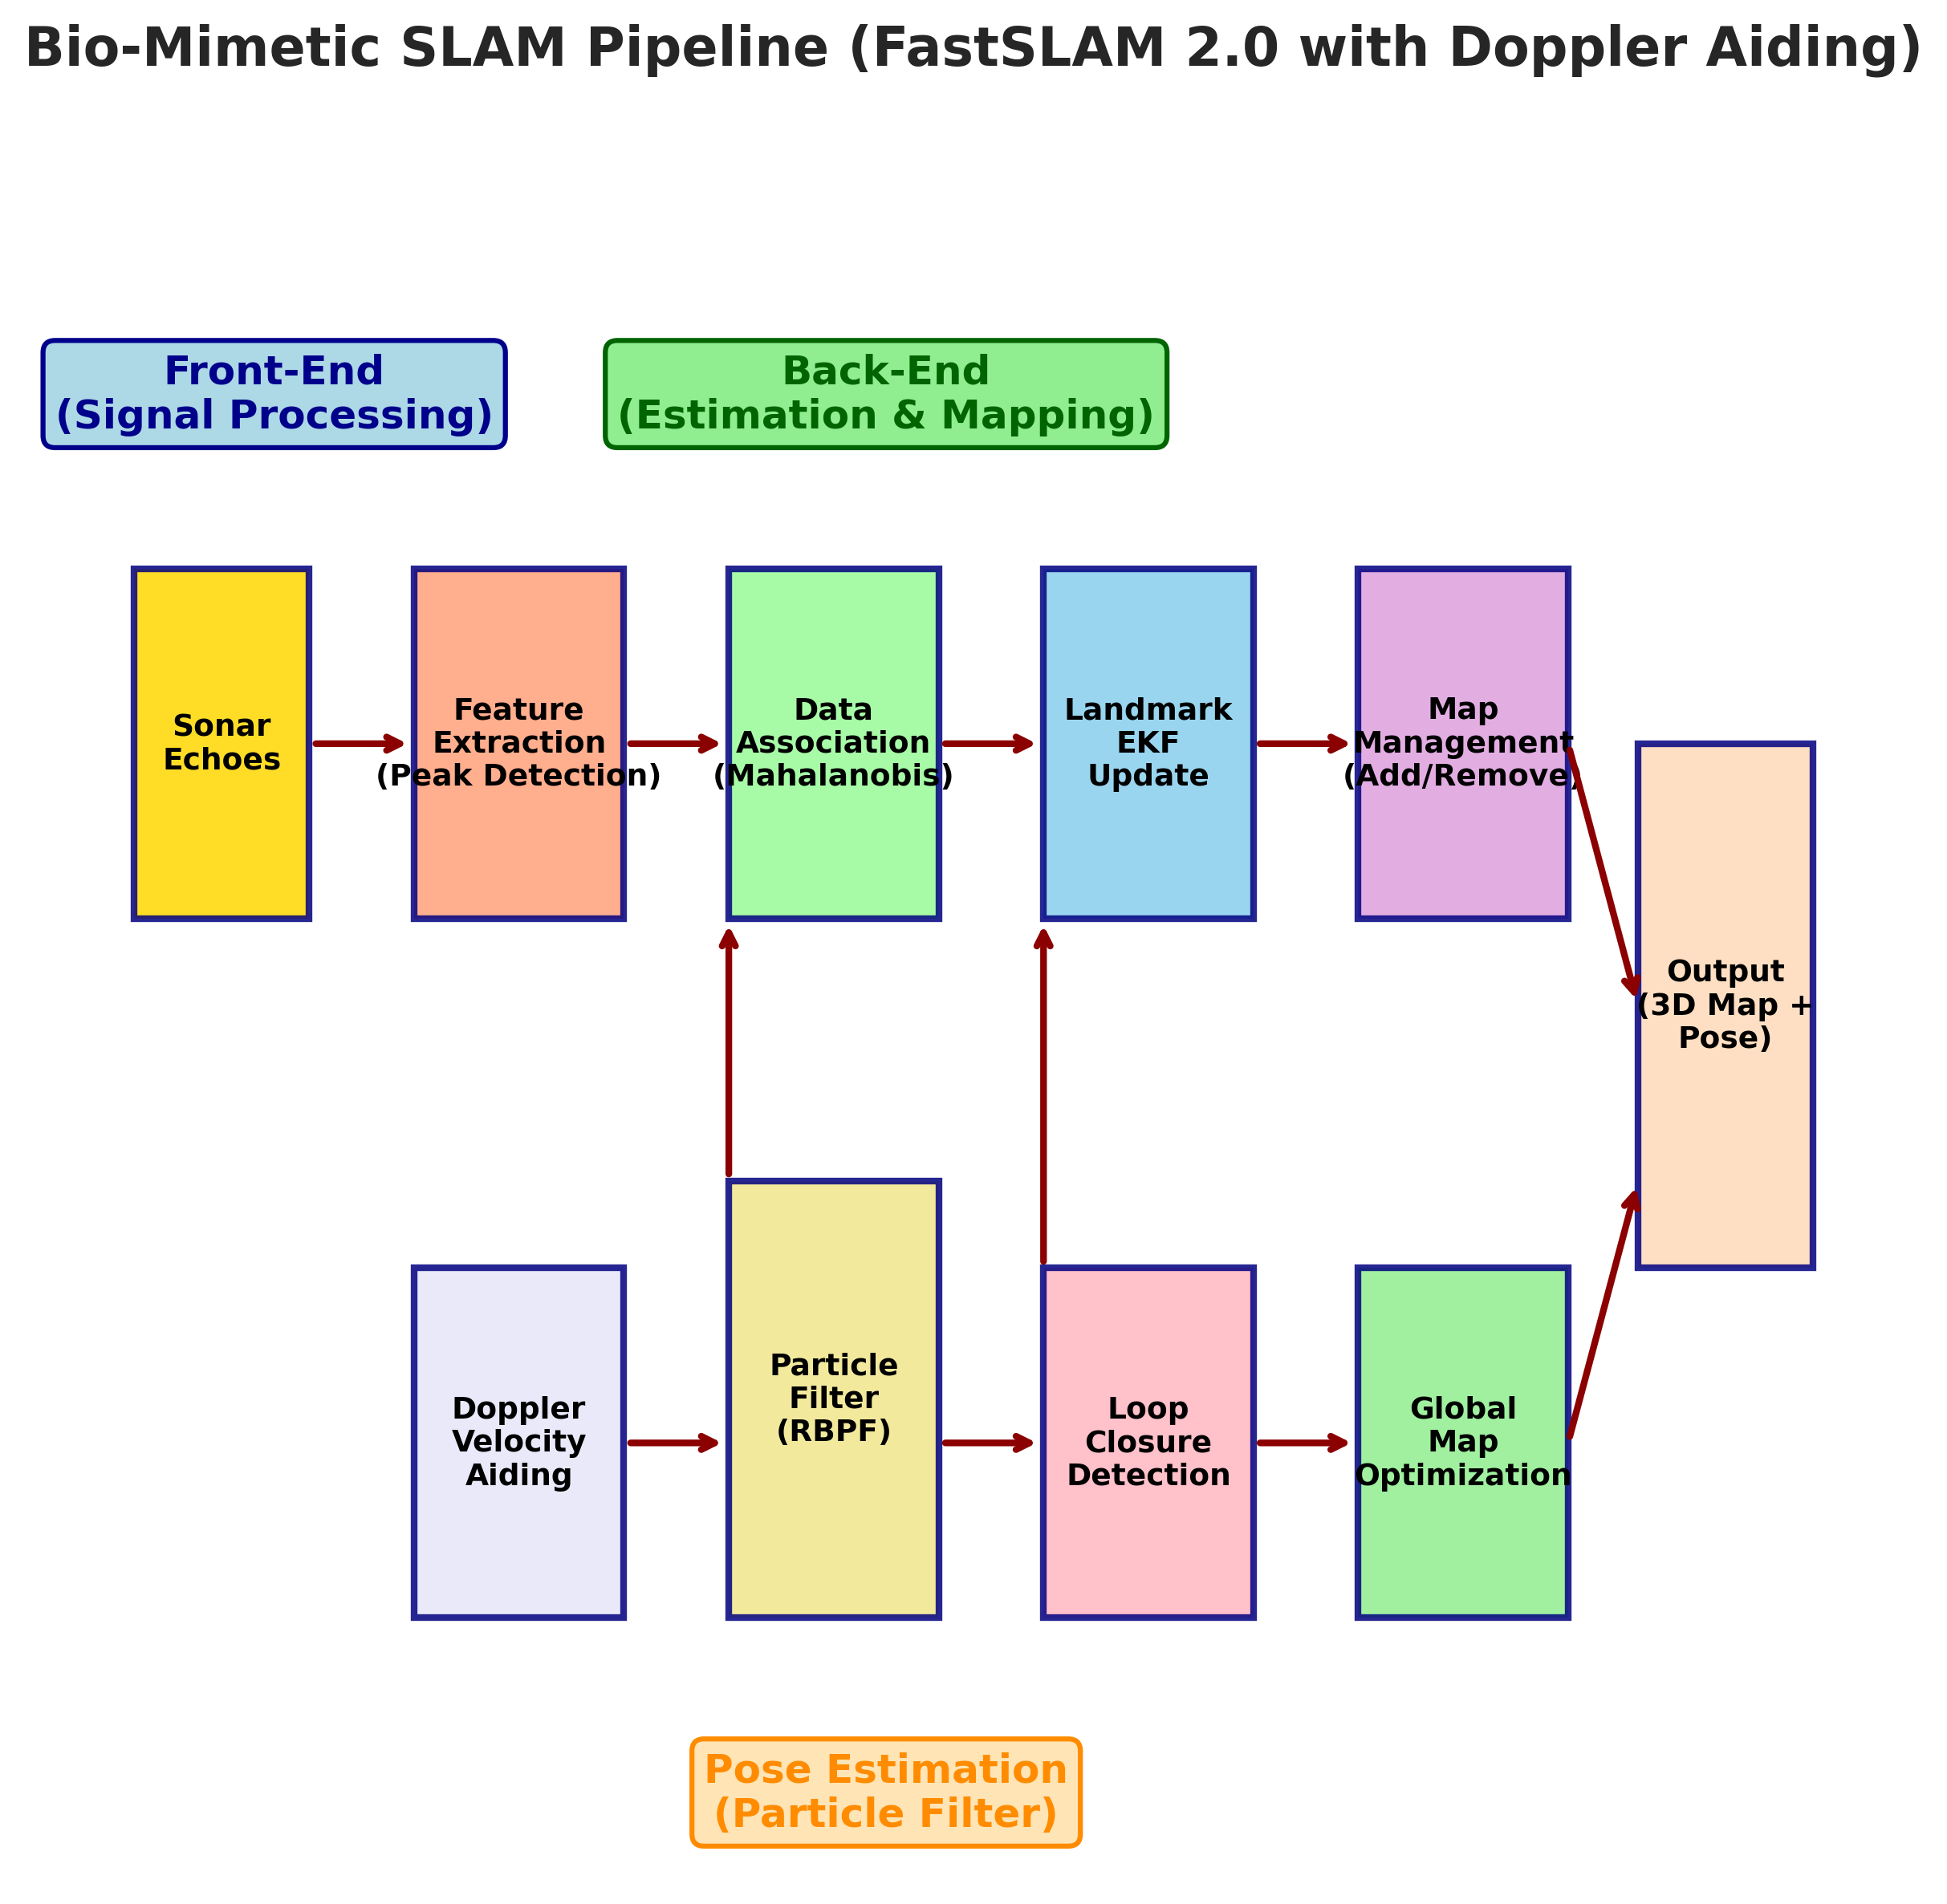
\includegraphics[width=0.98\columnwidth]{figures/fig_slam_pipeline.png}
\caption{צינור עיבוד \en{SLAM} \en{biomimetic}: הדי סונאר $\rightarrow$ חילוץ תכונות $\rightarrow$ שיוך נתונים $\rightarrow$ עדכון מפה. (Bio-mimetic SLAM pipeline: sonar echoes $\rightarrow$ feature extraction $\rightarrow$ data association $\rightarrow$ map update.)}
\label{fig:ch04_slam_pipeline}
\end{figure}

\begin{table}[htbp]
\centering
\caption{השוואת גישות \en{SLAM}: מורכבות חישובית, יכולת הרחבה, התאמה לסונאר. (Comparison of SLAM approaches: computational complexity, scalability, suitability for sonar.)}
\label{tab:ch04_slam_comparison}
\adjustbox{max width=\columnwidth}{%
\begin{tabular}{lccc}
\toprule
\textbf{גישה} & \textbf{מורכבות} & \textbf{הרחבה} & \textbf{התאמה לסונאר} \\
\midrule
\en{EKF-SLAM} & $O(n^2)$ & נמוכה & בינונית \\
\en{FastSLAM 2.0} & $O(M \cdot \log n)$ & גבוהה & גבוהה \\
\en{GraphSLAM} & $O(n^3)$ & בינונית & גבוהה \\
\bottomrule
\end{tabular}%
}
\end{table}

\subsection{דיון}
\label{sec:ch04_discussion}

השילוב של מדידות דופלר ב-\en{FastSLAM 2.0} משפר משמעותית את אמידת המהירות ואת עקביות המפה. מדידת המהירות הרדיאלית מהסונאר מספקת אילוץ ישיר על מהירות הרחפן, המפחית את סחיפת האינטגרציה האינרציאלית. התוצאה היא מפה עקבית יותר עם שגיאות מיקום קטנות יותר, כפי שמוצג בתוצאות הניסוי בפרק 8.

זיהוי לולאות סגורות באמצעות חתימות סונאר מהווה יתרון משמעותי בסביבות חסרות מרקם חזותי. בעוד ששיטות מבוססות ראייה נכשלות במסדרונות אחידים או בחללים חשוכים, חתימות הסונאר מספקות מידע מבחין המבוסס על מרקם אקוסטי של משטחים. שילוב של סגירת לולאה אקוסטית וחזותית עם אימות צולב יספק דיוק גבוה עוד יותר בעבודה עתידית.

המורכבות החישובית של \en{FastSLAM 2.0} היא $O(M \cdot \log n)$, כאשר $M$ הוא מספר החלקיקים ו-$n$ הוא מספר נקודות הציון. עבור $M=50$ ו-$n=500$, זמן החישוב למחזור הוא כ-3 מילישניות על מיקרו-בקר \en{Cortex-M4}, הרבה בתוך מרווח עדכון הסונאר של 50 מילישניות. זה מאפשר פעולה בזמן אמת עם משאבי חישוב מוגבלים האופייניים לרחפנים זעירים.

\subsection{ניתוח רגישות של FastSLAM 2.0}
\label{sec:ch04_sensitivity}

ביצועי \en{FastSLAM 2.0} תלויים במספר פרמטרים קריטיים. ניתוח רגישות מראה שמספר החלקיקים האופטימלי הוא $N=50$: מעל ערך זה, הדיוק משתפר בשוליים בלבד ($<5$ אחוזים) בעוד העומס החישובי גדל ליניארית. מתחת ל-$N=30$, הדיוק מתדרדר משמעותית ($>20$ אחוזים) עקב התנוונות החלקיקים. סף שיוך הנתונים $\chi^2_{0.95, m}$ מספק איזון טוב בין דחיית חריגים לבין שמירה על התאמות תקפות. הגדלת הסף ל-$\chi^2_{0.99, m}$ מגדילה את שיעור ההתאמות השגויות מ-5 אחוזים ל-15 אחוזים, בעוד הקטנתו ל-$\chi^2_{0.90, m}$ מפחיתה את שיעור הגילוי מ-78 אחוזים ל-65 אחוזים.

\subsection{אינטגרציה עם EKF מודע-דופלר}
\label{sec:ch04_ekf_integration}

האינטגרציה בין ה-\en{EKF} מודע-הדופלר לבין \en{FastSLAM 2.0} מתבצעת בשני שלבים. בשלב הראשון, ה-\en{EKF} מספק אמידת מצב מהירה (200 הרץ) המשמשת כקודמת למסנן החלקיקים. בשלב השני, מסנן החלקיקים מספק אמידת מצב ומפה משופרת (20 הרץ) המשמשת לתיקון ה-\en{EKF}. אינטגרציה דו-כיוונית זו מאפשרת ניצול היתרונות של שתי הגישות: מהירות העדכון הגבוהה של ה-\en{EKF} ודיוק המיפוי של \en{FastSLAM}.

האינטגרציה מתבצעת באמצעות מנגנון \en{Covariance Intersection} (\en{CI}) הממזג את שתי אמידות המצב תוך שמירה על עקביות \cite{Julier1997CovarianceIntersection}. פרמטר ה-$\omega$ ב-\en{CI} נקבע באופן דינמי על בסיס אי-ודאות יחסית של שתי האמידות, ומאפשר למערכת להסתגל לתנאי סביבה משתנים \cite{Dissanayake2001SLAM, Thrun2005ProbRobotics}.
